%! \usepackage{amsmath, amssymb, mathtools, braket}
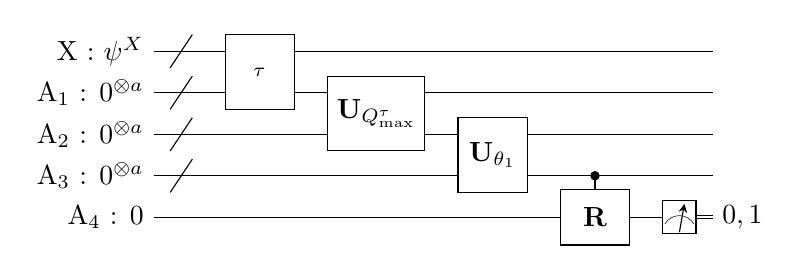
\begin{tikzpicture}[scale=1.000000,x=1pt,y=1pt]
\filldraw[color=white] (0.000000, -7.500000) rectangle (202.000000, 67.500000);
% Drawing wires
% Line 3: inputstate W \Ket{\psi}^X
\draw[color=black] (0.000000,60.000000) -- (202.000000,60.000000);
\draw[color=black] (0.000000,60.000000) node[left] {X : $\Ket{\psi}^X$};
% Line 4: qtau W \Ket{0}^{\otimes a}
\draw[color=black] (0.000000,45.000000) -- (202.000000,45.000000);
\draw[color=black] (0.000000,45.000000) node[left] {A$_1$ : $\Ket{0}^{\otimes a}$};
% Line 5: qtaunormalized W \Ket{0}^{\otimes a}
\draw[color=black] (0.000000,30.000000) -- (202.000000,30.000000);
\draw[color=black] (0.000000,30.000000) node[left] {A$_2$ : $\Ket{0}^{\otimes a}$};
% Line 6: theta W \Ket{0}^{\otimes a}
\draw[color=black] (0.000000,15.000000) -- (202.000000,15.000000);
\draw[color=black] (0.000000,15.000000) node[left] {A$_3$ : $\Ket{0}^{\otimes a}$};
% Line 7: cos W \Ket{0} {0,1}
\draw[color=black] (0.000000,0.000000) -- (190.000000,0.000000);
\draw[color=black] (190.000000,-0.500000) -- (202.000000,-0.500000);
\draw[color=black] (190.000000,0.500000) -- (202.000000,0.500000);
\draw[color=black] (0.000000,0.000000) node[left] {A$_4$ :   $\Ket{0}$};
% Done with wires; drawing gates
% Line 9: inputstate qtau qtaunormalized theta /
\draw (6.000000, 54.000000) -- (14.000000, 66.000000);
\draw (6.000000, 39.000000) -- (14.000000, 51.000000);
\draw (6.000000, 24.000000) -- (14.000000, 36.000000);
\draw (6.000000, 9.000000) -- (14.000000, 21.000000);
% Line 11: qtau inputstate G $\Or_\tau$ width=25 height=20
\draw (38.500000,60.000000) -- (38.500000,45.000000);
\begin{scope}
\draw[fill=white] (38.500000, 52.500000) +(-45.000000:17.677670pt and 19.091883pt) -- +(45.000000:17.677670pt and 19.091883pt) -- +(135.000000:17.677670pt and 19.091883pt) -- +(225.000000:17.677670pt and 19.091883pt) -- cycle;
\clip (38.500000, 52.500000) +(-45.000000:17.677670pt and 19.091883pt) -- +(45.000000:17.677670pt and 19.091883pt) -- +(135.000000:17.677670pt and 19.091883pt) -- +(225.000000:17.677670pt and 19.091883pt) -- cycle;
\draw (38.500000, 52.500000) node {$\Or_\tau$};
\end{scope}
% Line 12: qtaunormalized qtau G $\mathbf{U}_{Q_{\max}^{\tau}}$ width=35 height=20
\draw (80.500000,45.000000) -- (80.500000,30.000000);
\begin{scope}
\draw[fill=white] (80.500000, 37.500000) +(-45.000000:24.748737pt and 19.091883pt) -- +(45.000000:24.748737pt and 19.091883pt) -- +(135.000000:24.748737pt and 19.091883pt) -- +(225.000000:24.748737pt and 19.091883pt) -- cycle;
\clip (80.500000, 37.500000) +(-45.000000:24.748737pt and 19.091883pt) -- +(45.000000:24.748737pt and 19.091883pt) -- +(135.000000:24.748737pt and 19.091883pt) -- +(225.000000:24.748737pt and 19.091883pt) -- cycle;
\draw (80.500000, 37.500000) node {$\mathbf{U}_{Q_{\max}^{\tau}}$};
\end{scope}
% Line 13: theta qtaunormalized G $\mathbf{U}_{\theta_1}$ width=25 height=20
\draw (122.500000,30.000000) -- (122.500000,15.000000);
\begin{scope}
\draw[fill=white] (122.500000, 22.500000) +(-45.000000:17.677670pt and 19.091883pt) -- +(45.000000:17.677670pt and 19.091883pt) -- +(135.000000:17.677670pt and 19.091883pt) -- +(225.000000:17.677670pt and 19.091883pt) -- cycle;
\clip (122.500000, 22.500000) +(-45.000000:17.677670pt and 19.091883pt) -- +(45.000000:17.677670pt and 19.091883pt) -- +(135.000000:17.677670pt and 19.091883pt) -- +(225.000000:17.677670pt and 19.091883pt) -- cycle;
\draw (122.500000, 22.500000) node {$\mathbf{U}_{\theta_1}$};
\end{scope}
% Line 14: cos G $\mathbf{R}$ theta width=25 height=20
\draw (159.500000,15.000000) -- (159.500000,0.000000);
\begin{scope}
\draw[fill=white] (159.500000, -0.000000) +(-45.000000:17.677670pt and 14.142136pt) -- +(45.000000:17.677670pt and 14.142136pt) -- +(135.000000:17.677670pt and 14.142136pt) -- +(225.000000:17.677670pt and 14.142136pt) -- cycle;
\clip (159.500000, -0.000000) +(-45.000000:17.677670pt and 14.142136pt) -- +(45.000000:17.677670pt and 14.142136pt) -- +(135.000000:17.677670pt and 14.142136pt) -- +(225.000000:17.677670pt and 14.142136pt) -- cycle;
\draw (159.500000, -0.000000) node {$\mathbf{R}$};
\end{scope}
\filldraw (159.500000, 15.000000) circle(1.500000pt);
% Line 15: cos M
\draw[fill=white] (184.000000, -6.000000) rectangle (196.000000, 6.000000);
\draw[very thin] (190.000000, 0.600000) arc (90:150:6.000000pt);
\draw[very thin] (190.000000, 0.600000) arc (90:30:6.000000pt);
\draw[->,>=stealth] (190.000000, -5.400000) -- +(80:10.392305pt);
% Done with gates; drawing ending labels
\draw[color=black] (202.000000,0.000000) node[right] {${0,1}$};
% Done with ending labels; drawing cut lines and comments
% Done with comments
\end{tikzpicture}
